\subsubsection{\stid{4.16} ZFP: Compressed Floating-Point Arrays}

\paragraph{Overview} 

One of the primary challenges for Exascale computing is overcoming the
performance cost of data movement.  Through simulation, observation, and
experiments, far more data is being generated than can reasonably be stored
to disk and later analyzed without any form of data reduction.  Moreover,
with deepening memory hierarchies and dwindling per-core memory bandwidth
due to increasing parallelism, even on-node data motion between RAM and
registers makes for a significant performance bottleneck and primary source
of power consumption.

{\zfp} is a floating-point array primitive that mitigates this problem using
very high-speed, lossy (but optionally error-bounded) compression to
significantly reduce data volumes.  {\zfp} reduces I/O time and off-line
storage requirements by 1--2 orders of magnitude depending on accuracy
requirements, as dictated by user-set error tolerances.  Unique among data
compressors, {\zfp} also supports constant-time read/write random access to
individual array elements from compressed storage.  {\zfp}'s compressed arrays
can often replace conventional arrays in existing applications with minimal
code changes, allowing for instance the user to store tables of floating-point
data in compressed form that otherwise would not fit in memory, either using
a desired memory footprint or a prescribed level of accuracy.  When used in
numerical computations, {\zfp} arrays provide a fine-grained knob on precision
while achieving accuracy comparable to IEEE floating point at half the
storage, reducing both memory usage and bandwidth.

This project is extending {\zfp} to make it more readily usable in an Exascale
computing setting, by parallelizing it on both the CPU and GPU while ensuring
thread safety; by providing bindings for several programming languages (C,
C++, Fortran, Python); by adding new functionality, e.g., for unstructured
data and spatially adaptive compressed arrays; by hardening the software and
adopting best practices for software development; and by integrating {\zfp}
with a variety of ECP applications, I/O libraries, and visualization and data
analysis tools.


\paragraph{Key  Challenges}

There are several challenges to overcome on this project with respect
to implementing compressed floating-point arrays:
%
\begin{itemize}
\item \textbf{Data dependencies}.  Compression by its very nature removes
redundancies, often by deriving information from what has already been
(de)compressed and learned about the data.  Such data dependencies can
usually be resolved only by traversing the data in sequence, thus
complicating random access and parallelism.

\item \textbf{Random access}.  For inline compression, on-demand random
access to localized pieces of data is essential.  However, compression
usually represents large fixed-length records using variable-length
storage, which complicates random access and indexing.

\item \textbf{Parallelism}.  Manycore architectures allow for massively
concurrent execution over millions or billions of array elements.
Yet compression is usually a process of reducing such multidimensional
arrays to a single-dimensional
sequence of bits, which requires considerable coordination among parallel
threads of execution.

\item \textbf{Unstructured data}.  Unstructured data, such as independent
particles and arbitrarily connected nodes in a mesh, has no natural
ordering, repeated structure, or regular geometry that can be exploited
for compression.

\item \textbf{Performance}.  For inline compression to be useful, both
compression and decompression have to be extremely fast (simple), yet
effective enough to warrant compression.  Moreover, the complexities of
compression must be hidden from the user to promote adoption, while allowing
sufficient flexibility to support essentially arbitrary data access patterns.
\end{itemize}
%
These challenges often suggest conflicting solutions and are further
complicated by the extreme demands of Exascale computing applications.

\paragraph{Solution Strategy}


{\zfp} is unique in supporting read and write random access to
multidimensional data, and was designed from the outset to address
some of the above challenges.  The following strategies are employed on
this project to overcome the remaining challenges:
%
\begin{itemize}
\item \textbf{Partitioning}.  $d$-dimensional arrays are partitioned
into small, independent blocks of $4^d$ scalars each.  This enables both
fine-grained random access and a large degree of data parallelism.

\item \textbf{Fixed-size storage}.  Instead of storing fixed-precision
values using variable-size storage, {\zfp} uses fixed-size storage to
represent values at the greatest precision afforded by a limited
bit budget.

\item \textbf{Adaptive storage}.  For applications that demand error
tolerances, this project is developing adaptive representations that
allocate bits to where they are most needed, which involves efficient
management of variable-length records that might expand and shrink in
size over time.

\item \textbf{Parallelism}.  OpenMP and CUDA implementations of {\zfp}
have been developed that exploit fine-grained data parallelism.
Opportunities for task parallelism have also been identified.

\item \textbf{Preconditioning}.  The irregularity and unpredictability
of unstructured data is improved using \emph{preconditioners} that
``massage'' the data to make it more amenable to compression by {\zfp}.
Strategies include sorting, binning, structure inference, transposition,
pre-transforms like wavelets, etc.

\item \textbf{Abstraction}.  Concrete details about compression, caching,
parallelism, thread safety, etc., are abstracted away from the user by
providing high-level primitives that make {\zfp} arrays appear like
uncompressed arrays, in part via C++ operator overloading.  We are
designing classes and concepts commonly available for uncompressed arrays,
such as proxy references and pointers into compressed storage that act
like their uncompressed counterparts; views into and slices of arrays;
and iterators compatible with STL algorithms.  Such primitives make it
easier to write generic code for which {\zfp} arrays may easily be
substituted for uncompressed arrays.
\end{itemize}

\paragraph{Recent Progress}

This project has made progress on several fronts over the past six months to
make the {\zfp} software~\cite{zfp-code} more Exascale ready and capable.
The 0.5.4 release of {\zfp} adds array slicing and views into arrays,
which enable thread-safe concurrent read and write access.  New in this
release is also a CUDA implementation of fixed-rate compression and
decompression.  Our CUDA implementation has undergone several rewrites to
improve performance, culminating in a 150~GB/s compression throughput on an
NVIDIA~V100 GPU.  Also new in {\zfp}~0.5.4 is support for compressing 4D
data and C bindings to {\zfp}'s C++ compressed array primitives.

Further developments since the fall release include work on Fortran
and Python bindings to {\zfp}'s high-level compression API---efforts
that are both nearing completion.
Meanwhile, we have devised several independent candidates for lossless
compression within {\zfp} that are being evaluated.
%, including a generalization of iterative
%refinement; a sieve that distinguishes {\zfp} blocks that can be
%compressed losslessly from those that should be stored verbatim; as well
%as a new decorrelating transform that does not incur round-off error.
%We are currently evaluating these strategies and will select one for
%inclusion in the next {\zfp} release.
Although not designed for compression of unstructured data, we have
applied {\zfp} to particle-based data
%from molecular dynamics,
%cosmology, and particle-in-cell codes, and to data attached to
%unstructured meshes
by first ``preconditioning'' it via local
sorts that increase autocorrelation.  We found this strategy largely
ineffective, however.
A more successful preconditioner is to pass structured data through
a wavelet transform, which we found to improve accuracy by as much as
an order of magnitude for the same storage cost.

Finally, we have been working with ECP tools and applications to integrate
{\zfp} compression.  One effort that is wrapping up is support in VTK-m for
compressing and decompressing multidimensional arrays.  We are also
working with CEED to develop a {\zfp}-based format for high-order
finite elements.

The results of our R\&D efforts have been documented through
publications~\cite{zfp-isc2017,zfp-jsm2017}, and significant efforts have
been made to reach out to customers and the HPC community at large through
one-on-one interactions and tutorials, both at ECP meetings and
conferences~\cite{zfp-isc2017-tut,zfp-sc2017-tut,zfp-ep2018-tut,zfp-sc2018-tut}.

\noindent
\begin{minipage}[t]{3.75in}
\paragraph{Next Steps}

Efforts are underway to develop compressed array primitives that support
spatially adaptive variable-rate compression and that allocate bits to regions
where they are most needed.
%, for example, to meet a uniform error tolerance or precision.
Two separate efforts are being pursued to support read-only arrays, e.g., for
static tables and simulation results, and mutable arrays for which blocks may
expand or shrink in compressed size over time.  We are also considering
changes to the main compression CODEC to support new features that are being
added to {\zfp}, and we will be working toward filling gaps in the Cartesian
product feature space (array dimensionality, scalar type, programming
language, execution policy, etc.).

\end{minipage}%
\hspace*{0.125in}%
\begin{minipage}[t]{2.625in}
\vspace{0pt}%
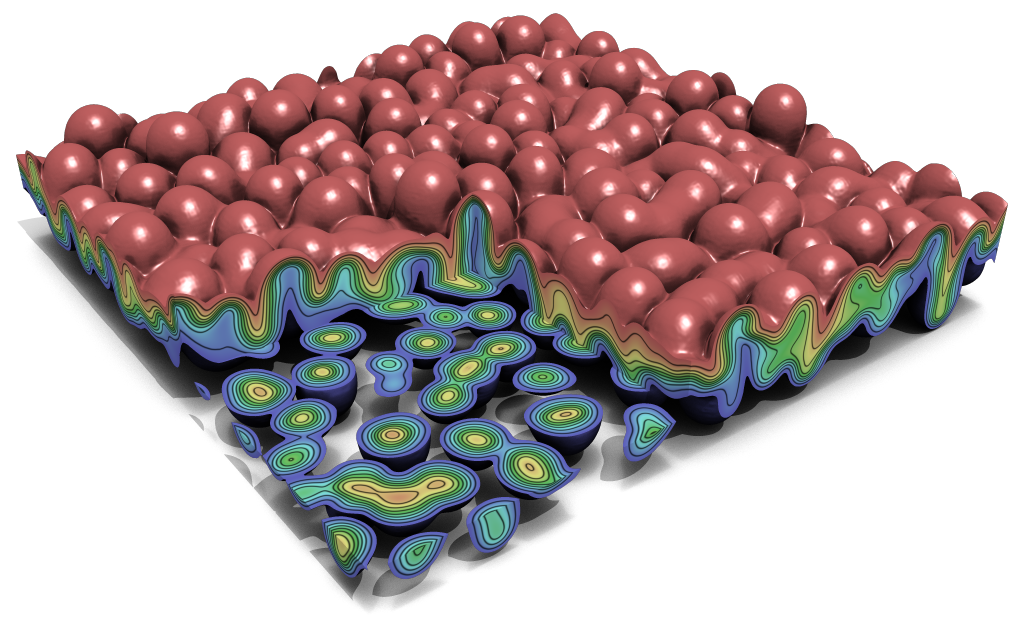
\includegraphics[width=\columnwidth]{projects/2.3.4-DataViz/2.3.4.16-ALPINE-ZFP/ZFP}%
\vspace{-2ex}%
\captionof{figure}{240:1 {\zfp} compressed density field.}%
\label{fig:zfp-result}%
\end{minipage}
